\documentclass[../../main.tex]{subfiles}

% 

\begin{document}
\chapter{Urýchľovače nabitých častíc}

Na štúdium vlastností, štruktúry a interakcií elementárnych častíc, výrobu umelých rádionuklidov, ako aj na aplikácie v rôznych oblastiach vedy a techniky je treba použiť častice urýchlené na vysoké kinetické energie. Keďže prírodné rádioaktívne látky poskytujú obmedzenú intenzitu a hlavne energiu emitovaných častíc, je nutné sa obrátiť k umelému urýchľovaniu častíc. Prístroje, ktoré nám to dovoľujú, sa nazývajú urýchľovače častíc.

Umelo urýchliť dokážeme iba stabilné elektricky nabité častice, zatiaľčo častice bez náboja alebo krátko žijúce častice (napr. pióny, hyperóny) možno získať sekundárne interakciami urýchlených nabitých častíc s ďalšími časticami vo vhodnom terčíku (rozpadom častíc sekundárneho zväzku možno získať zväzky terciálne, napr. $\nu_e$ či $\nu_\mu$). Vlastné urýchľovanie nabitých častíc spôsobuje elektrické pole (s intenzitou $\vec{E}$) svojim silovým pôsobením na náboj $\vec{F}_e=q\vec{E}$, magnetické pole sa v urýchľovačoch využíva na zmenu dráhy nabitých častíc a tiež zaisťuje fokuzáciu zväzku.

Nárast energie urýchľovanej častice za jednotku času je daný vzťahom
\begin{equation}
\dfrac{\mathrm{d}E}{\mathrm{d}t}=Ze\vec{v}\cdot\vec{\epsilon}
\end{equation}
kde $\vec{\epsilon}$ je vektor intenzity elektrického poľa. V rezonančných urýchľovačoch elektrické pole zabezpečuje ešte fázovanie zväzku.

Uhlová rýchlosť $\omega_c$ nazývaná cyklotrónová frekvencia v magnetickom poli je daná vzťahom
\begin{equation}
\omega_c=\dfrac{v}{R}=\dfrac{qB}{m}=\dfrac{qB}{m_0\gamma}=\dfrac{qBc^2}{E}.
\end{equation}

Dôležitou vlastnosťou urýchľovačov je ich luminozita. Intenzita, s akou prebiehajú interakcie urýchlených častíc, závisí na hustote ich toku. Charakterizuje sa práve pomocou veličiny zvanej luminozita $L\:\unit{[cm^{-2}s^{-1}]}$, čo je počet častíc na jednotku plochy za jednotku času. Na veľkých urýchľovačoch sa dosahuje luminozita $L\approx 10^{31}$ až $10^{33}\:\unit{cm^{-2}s^{-1}}$.

Početnosť produkovaných častíc z interakcií s účinným prierezom $\sigma$ dokážeme určiť podľa vzťahu $R=\sigma L$.

Budeme predpokladať, že zväzky sú tvorené malými valcovými zhlukmi (\textit{bunches}) častíc s priečnym prierezom $S$, ktoré sú rovnomerne rozprestrené v oboch smeroch pozdĺž urýchľovacej trubice. Zhluky sa v oblasti experimentu zrážajú s frekvenciou $f_B$, hustota toku častíc v oblasti experimentu cirkulujúcich v pravotočivom zmysle v kruhovom urýchľovači je $j_R=f_B\frac{N_R}{S}$. Počty častíc v zhlukoch krúžiacich v pravotočivom (resp. ľavotočivom) zmysle sú $N_R$ (resp. $N_L$). Potom pre luminozitu kruhového urýchľovača platí vzťah
\begin{equation}
L=f_B\dfrac{N_RN_L}{S}
\end{equation}

Keďže všetky pozorované udalosti v mikrosvete sú nepriame, spôsoby štúdia mikrosveta sa obmedzujú na rozpady nestabilných mikroobjektov (premena $\alpha$, $\beta$, samovoľné štiepenie) a na realizáciu zrážkových procesov. K realizácii zrážkových procesov je potreba zdroja častíc, terčíkov a detektorov.

\section{História}

História urýchľovačov siaha až do začiatku 20. storočia k Ernestovi Rutherfordovi. Tomu sa v roku 1919 podarilo ožarovaním jadier dusíku alfa časticami premeniť dusík na kyslík. Bola to nielen prvá jadrová reakcia, ale aj prvá transmutácia prvku, čo bol večný sen alchymistov. 

Behom ďalších rokov sa vedci snažili rozbíjať atómové jadrá. Tu sa objavila prvá iniciatíva využiť urýchlené častice. Rutherford si uvedomil, že prírodné alfa častice sú príliš neúčinné, a že potrebuje umelé zdroje, ktoré poskytujú vyššie energie, ako prirodzená rádioaktivita. V roku 1924 prišiel do jeho laboratória John Cockroft a spoločne hľadali spôsob, akým urýchliť protóny elektrickým poľom s vysokým napätím. 

V roku 1929 skonštruoval Robert Jemison Van de Graaff prvý funkčný prototyp generátoru vysokého napätia. V roku 1931 získal na svoj generátor patent. V tom istom roku zostrojil lineárny urýchľovač dlhý 2 metre a dosahujúci energie 1,5 MeV. Generátor vtedy produkoval napätie približne milión voltov, pričom bol vyrobený z materiálu za 90 dolárov. 

V roku 1932 sa Johnovi Cockroftovi a Ernestovi Waltonovi podarilo zostrojiť lineárny urýchľovač na inom princípe, než na ktorom pracoval Van de Graafov stroj. Zdrojom napätia sa stal tzv. kaskádový generátor. Aj ich sprevádzali ťažkosti pri stavbe nového urýchľovača, najmä pri vytvorení vákuového systému. Ich práca znamenala obrovský posun vpred. Vedci sa totiž domnievali, že na rozbitie jadier bude treba veľmi veľká energia. Ruský fyzik George Gamow teoreticky sformuloval predpoklad tunelového efektu (založeného na kvantovej mechanike), ktorý hovorí, že do jadra sa môžu dostať protóny aj s omnoho menšou energiou.

Na vývoji urýchľovačov sa podieľal aj Rolf Wideroe. Tento nórsky inžinier prišiel už v roku 1922 s návrhom kruhového urýchľovača - bevatronu. V roku 1926 predložil tento návrh ako svoju dizertačnú prácu, no tá bola zamietnutá rovnako ako jeho žiadosť na patentovom úrade. Pre nedostatočné teoretické prepracovanie zostrojil v roku 1927 nefunkčný prototyp. Aj kvôli týmto nezdarom prešiel ku stavbe lineárneho urýchľovača. Ešte v tom roku sa mu podarilo zostrojiť prvý funkčný lineárny urýchľovač. Jeho prevratné myšlienky inšpirovali mnoho vedcov, napr. Ernesta Lawrenca.

Ernest Lawrence dostal prezývku \quotedblbase drtič atómov\textquotedblright . Spoločne so svojim študentom Davidom Sloanom zostrojili v roku 1931 prvý rezonančný lineárny urýchľovač, v ktorom sa postupne elektricky nabité častice urýchľujú pomocou vysokofrekvenčného elektromagnetického poľa. Lawrence bol inšpirovaný článkom, ktorý Wideroe publikoval. Síce nevedel nemecky, ale z obrázku pochopil hlavnú myšlienku. 

V roku 1931 došlo k významnej modifikácii na kruhový urýchľovač, čo bol prvý cyklotrón. Lawrence je nositeľom Nobelovej ceny za tento vynález a predovšetkým za ním získané výsledky v oblasti umelých rádioaktívnych prvkov. Jednalo sa o malý stroj s priemerom 10 cm, protónom sa vtedy podarilo udeliť energiu 80 keV. Vďaka rýchlemu vývoju mali cyklotróny behom dvoch rokov priemer okolo 80 cm a protóny získavali energiu 1,2 MeV. Pomocou cyklotrónu mohol byť atóm rozbitý skôr, než sa to podarilo Cockroftovi a Waltonovi, no Lawrence svoj prístroj sprvu nepoužíval na fyzikálne pokusy.

Behom tridsiatych rokov boli v Berkeley uvedené do prevádzky stále väčšie cyklotróny a stávali sa užitočnejším nástrojom aj pre iné vedecké odvetvia. Jednou z oblastí, ktorou sa Lawrence zaoberal, bola príprava rádioaktívnych izotopov pre medicínu a biológiu.

V roku 1940 zostrojil Donald Kerst magnetický indukčný urýchľovač elektrónov - betatron. Princíp indukčného urýchľovania spracoval už v dvadsiatych rokoch Wideroe. Aj Kerstove experimenty sa stretávali s problémami, jeho prístroj\footnote{jeho prístroj niesol niekoľko názvov, napr. Rheotron, Inductron, Super-X-Ray Machine, Cosmic Ray Machine, Ausserordentlichhochgeschwindigkeitelektronenentwickelndenschwerarbeitsbeigollitron.} tak namiesto pôvodných 400 dolárov stál 2000 dolárov. Postupne sa však ukázalo, že cyklotrónová technika naráža na technické problémy, ktoré limitujú energiu dosiahnutú na tomto type urýchľovača na cca 20 MeV. Na dosiahnutie vyšších energií museli byť vynájdené nové typy urýchľovacej techniky.

Po druhej svetovej vojne vynašiel Lawrencov kolega Edwin McMillan nový typ urýchľovača - synchrotrón. V ňom sa častice nepohybujú po špirále, ale po kruhovej dráhe. Prvý protónový synchrotron pracoval v BNL (Brookhaven National Laboratory) neďaleko New Yorku. V roku 1952 dosiahol energiu až 3 GeV. Bol to prvý urýchľovač, ktorý poskytoval častice s energiou porovnateľnou s kozmickým žiarením a preto sa mu tiež hovorilo aj kozmotron. V roku 1955 vyprodukovali fyzici na tomto urýchľovači antiprotóny. Kozmotronu patrilo prvenstvo až do doby, než v Berkeley v roku 1954 uviedli do prevádzky Bevatron\footnote{Názov pochádza zo skratky Billions of electronvolts - BeV} s energiou 6 GeV.

V decembri 1949 sa vo Švajčiarsku konala konferencia spojených národov, ktorá sa zaoberala biednym stavom vedy v povojnovej Európe. Vedci sa behom vojny rozutekali po celom svete a centrum výskumu sa presunulo do USA. Tu po prvýkrát zaznela výzva francúzskeho fyzika Louisa de Broglieho, ktorý doporučil založiť medzinárodné výskumné laboratórium. O 6 mesiacov neskôr sa neďaleko Ženevy zrodil CERN. S výstavbou sa začalo v roku 1954. Rusi nechceli zaostávať za zbytkom sveta a tak po vzore CERNu založili Spojený ústav jadrových výskumov v meste Dubna. V roku 1956 bola podpísaná zmluva, ktorá definuje tento ústav ako medzinárodnú inštitúciu s niekoľkými členskými štátmi. V roku 1957 tu bol uvedený do prevádzky synchrofázotron, ktorý dosahoval svetový rekord 10 GeV.

Studená vojna na poli vedeckom znamenala predovšetkým konkurenciu medzi CERNom, BNL a Dubnou. Hlavným cieľom CERNu bolo postaviť protónový synchrotrón PS s energiou 28 GeV, najväčší urýchľovač tej doby, a prekonať tak ruské prvenstvo. BNL plánovala výstavbu urýchľovača AGS (Alternativ Gradient Synchrotron), ktorý mal dosiahnuť energiu 30 GeV a získať tak rekord. V roku 1959 po spustení synchrotrónu v CERNe Európa tento závod vyhrala. Rivalita medzi laboratóriami bola taká, že dokonca sovietsky kolegovia poslali fľašu vodky určenú špeciálne na túto príležitosť do CERNu. Fľaša kolovala po úspešnom spustení kontrolnou miestnosťou. Potom vedúci skupiny PS, John Adams, uložil do prázdnej fľaše záznamy, ktoré dokumentovali dosiahnutý úspech, a nechal fľašu poslať naspäť do Ruska.

V roku 1967 poskytol prvý zväzok lineárny urýchľovač SLAC (Stanford Linear Accelerator Center) v Berkeley. Veľký zlom v ich práci nastal, keď posunuli detektory ďalej od línie zväzku, aby mohli pozorovať elektróny, ktoré zmenili smer. K údivu všetkých bolo týchto elektrónov veľmi veľa. V tej dobe tu pôsobil Richard Feynman a James Bjorker. Vďaka ich prevratnému experimentu dospeli k záveru, že vnútri nukleónu sa nachádzajú nabité bodové objekty.

Ďalším americkým centrom zaoberajúcim sa urýchľovaniu častíc bol Fermilab (Fermi National Accelerator Laboratory). Bol založený v roku 1967 a prvým riaditeľom sa stal Robert Wilson, vynálezca hmlovej komory. Od roku 1983 sa tu nachádzal najväčší urýchľovač sveta - Tevatron. Ten so svojim obvodom 6,28 km dosahoval energiu 980 GeV. K najvýznamnejším objavom patrí objav charmonia, b kvarku, t kvarku a $\tau$ neutrína.

\section{Zdroje častíc na urýchľovanie}

Zdroj urýchľovaných častíc (iónový zdroj) emituje do štartovacieho miesta urýchľovacieho systému požadovaný druh častíc ako sú elektróny, protóny či ťažšie ióny. V najjednoduchšom prípade sa jedná o ionizačnú trubicu obsahujúcu príslušný zriedený plyn (napr. vodík), kde v tlejúcom výboji medzi katódou a anódou (pri napätí stovky až tisíce voltov) vznikajú ióny a tie sú pomocou tenkej kapiláry vedené elektródou do urýchľovacieho systému.

Na získanie ťažkých iónov sa používa výboj v zriedenom plyne (obsahujúcom príslušný prvok) pri dostatočne vysokom napätí, aby dochádzalo k ionizácii aj na K-šupke. Vznikajú pritom ióny s rôznym stupňom ionizácie, z ktorých je treba požadované jadrá (ióny s najvyšším stupňom ionizácie) odseparovať pomocou magnetického poľa a zaviesť ich do urýchľovacieho systému.

Pre urýchľovače elektrónov je zdrojom obyčajná žeravá katóda (termoemisia elektrónov) opatrená vhodnými urýchľujúcimi a fokuzujúcimi anódami.

Zložitejšie sa pre urýchlenie získavajú antičastice. Napr. pozitróny sa získavajú ostreľovaním terčíku z materiálu s vysokým protónovým číslom $Z$ urýchlenými elektrónmi, pričom elektromagnetickou interakciou v poli jadier vznikajú okrem iného aj pozitróny. Podobne antiprotóny je nutné získavať ostreľovaním vhodného terčíku protónmi urýchlenými na energie vyššie než 3 GeV, kedy dochádza k reakciám $p+p\rightarrow 2p+p+\bar{p}$.

Pri veľkých urýchľovačoch s vysokými energiami sa ako zdroje častíc k urýchleniu niekedy používajú injektory - do hlavnej komory sú predurýchlené častice vstrekované pomocným lineárnym či kruhovým urýchľovačom (s energiou v rádoch MeV, prípadne GeV) a následne urýchľované na požadovanú vysokú energiu.

\section{Injekcia častíc do storage ringu}

Častice vyrobené v zdroji a predurýchlené lineárnym urýchľovačom je treba vstreknúť do synchrotrónu, ktorý ich ďalej urýchli. To možno spraviť buď pomocou pulzných magnetov alebo - v špeciálnych prípadoch - pomocou vstrekovania cez stripping fóliu. Vďaka urýchľovacím vysokofrekvenčným dutinám môže byť na obvode synchrotrónu umiestnené iba určité množstvo zhlukov častíc. Pokiaľ sú všetky tieto pozície zaplnené zhlukmi na osi zväzku, nemožno už na os zväzku ďalšie zhluky pridať. V tejto súvislosti hovoríme o zaplnenom pozdĺžnom fázovom priestore urýchľovača.

Keby sme na navedenie zhluku na dráhu v synchrotróne použili magnet s konštantnou magnetickou indukciou, došlo by k tomu, že vstrekovaný zhluk by sa síce dostal na správnu dráhu, ale zhluky v urýchľovači už cirkulujúce by z nej boli vychýlené a dopadli by na stenu zväzkovej trubice. Pomocou pulzného magnetického poľa pôsobiaceho iba počas doby preletu vstrekovaného zhluku sa tomuto problému môžeme vyhnúť, čo je znázornené na obr. \ref{em2:img:injekcia1}.

\begin{figure}[h]
\centering
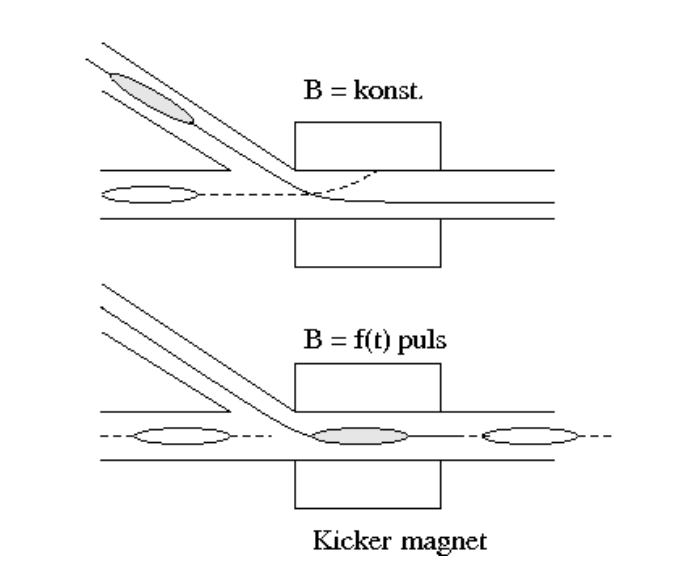
\includegraphics[width=0.5\textwidth]{em2-injekcia1.png}
\caption{Injekcia častíc do urýchľovača, zapĺňanie pozdĺžneho fázového priestoru.}
\label{em2:img:injekcia1}
\end{figure}

Pokiaľ potrebujeme pridať do synchrotrónu ďalšie zhluky častíc, môžeme využiť aj priečny fázový priestor, do ktorého možno umiestniť niekoľko zhlukov mimo os zväzku. Tento postup môžeme realizovať pomocou sústavy magnetov znázornenej na obr. \ref{em2:img:injekcia2}. Na obrázku je znázornené aj postupné plnenie v priečnej rovine.

\begin{figure}[h]
\centering
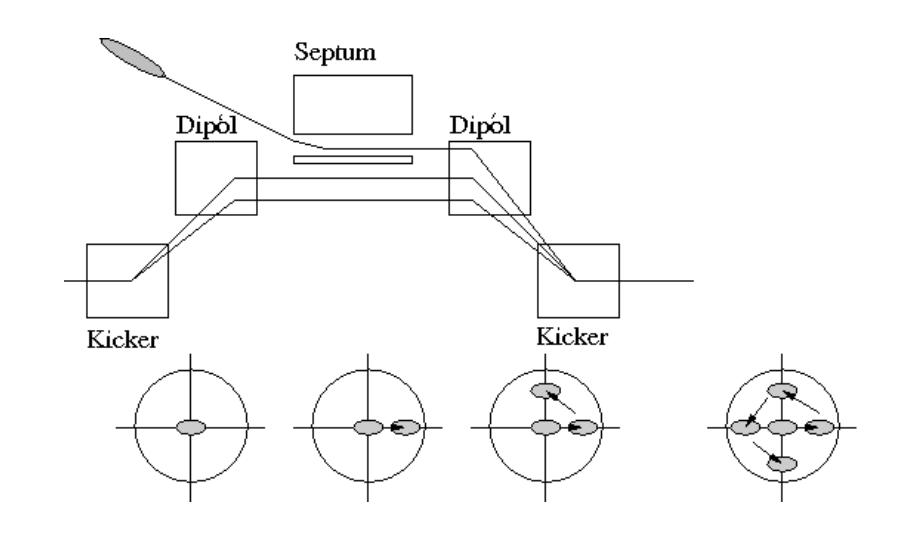
\includegraphics[width=0.7\textwidth]{em2-injekcia2.png}
\caption{Plnenie priečneho fázového priestoru urýchľovača.}
\label{em2:img:injekcia2}
\end{figure}

Protóny môžeme injektovať pomocou stripping fólie. Negatívne vodíkové ióny sú vstreknuté do konštantného dipólového magnetického poľa, ktoré v našom prípade na obr. \ref{em2:img:injekcia3} zatáča doľava. Po prelete stripping fóliou sú odtrhnuté oba elektróny a ďalej pokračuje iba kladný protón. Po obehu synchrotrónom sa protón dostáva do poľa prvého magnetu, ktorý ho vďaka pozitívnemu náboju zatáča doprava a dopraví ho na rovnakú dráhu ako vstrekovaný ión.

\begin{figure}[h]
\centering
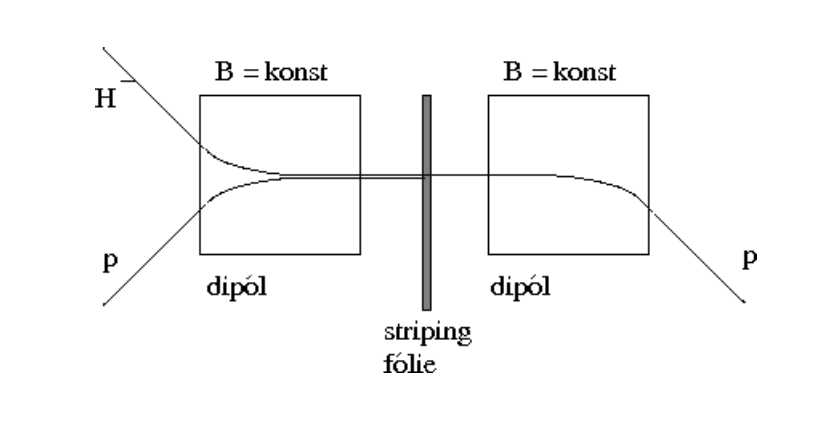
\includegraphics[width=0.6\textwidth]{em2-injekcia3.png}
\caption{Plnenie urýchľovača cez stripping fóliu.}
\label{em2:img:injekcia3}
\end{figure}

\section{Zrážače}

Ak dopadá urýchlená častica na pevný a nepohyblivý terčík a tam sa zrazí s ďalšími časticami alebo jadrom, spotrebuje sa na vlastnú interakciu v skutočnosti len malá časť kinetickej energie nalietavajúcej častice, pretože podľa zákona akcie a reakcie sa časť energie dopadajúcej častice premení na kinetickú energiu odrazenej častice a novo vzniknutých častíc. Pre výsledok interakcie je dôležitá kinetická energia v ťažiskovej sústave oboch častíc - len tá sa skutočne spotrebuje na vlastnú interakciu.

Podstatné zvýšenie efektívnej energie interakcie môžeme dosiahnuť tým, že nalietavajúca a terčíková častica sa budú pohybovať oproti sebe s porovnateľne veľkými kinetickými energiami. Obe takéto častice sa potom po zrážke prakticky zastavia a skoro celá ich kinetická energia sa môže využiť na vlastnú interakciu a tvorbu nových častíc. V tom spočíva metóda protichodných\footnote{česky vstřícných} zväzkov bez použitia klasického terčíku - obe častice, ktorých interakcie chceme skúmať, sa urýchlia na vysoké energie a v protichodných zväzkoch sa púšťajú oproti sebe tak, aby sa vzájomne čelne zrážali a interagovali.

Výhodou protichodných zväzkov je veľká hodnota energie, ktorá sa využije na vlastnú interakciu a tiež to, že experimentálna aparatúra je umiestnená okolo miesta zrážky (tzv. 4$\pi$ geometria). Nevýhodou je to, že nemôžeme formovať sekundárne zväzky, naviac prevedenie experimentov využívajúcich protichodné zväzky je podstatne pomalšie ako experimenty pracujúce s pevnými terčíkmi (pevný terčík totiž obsahuje viac častíc ako zväzok).

Oba zväzky sa urýchľujú buď v jednej trubici (napr. elektrón-pozitrónové zväzky), alebo v dvoch rôznych trubiciach. V danom mieste urýchľovacieho prstenca sa oba zväzky urýchlených častíc, letiacich opačným smerom oproti sebe, pôsobením magnetického poľa fokusujú a navedú sa tak, aby sa čelne zrážali. Prístroje tohto druhu sa nazvajú zrážače (\textit{collidery}) a umožňujú študovať interakcie častíc s podstatne vyššími efektívnymi energiami ako klasické urýchľovače s pevnými terčíkmi. Miesto, kde dochádza k interakciám - interakčná oblasť - je obklopené zložitým detekčným systémom pre detailné štúdium sekundárnych častíc. Zrážače sa používajú iba na bádateľský výskum interakcií častíc s vysokou energiou za vzniku nových exotických častíc.   

\section{Lineárne urýchľovače}

Lineárne urýchľovače urýchľujú nabité častice pôsobením elektrického poľa behom ich pohybu po priamej dráhe. Môžeme ich rozdeliť na elektrostatické a vysokofrekvenčné. 

Výhody lineárnych urýchľovačov oproti kruhovým sú najmä: jednoduchšia stavba, netreba mohutné magnety, jednoduchosť injekcie a extrakcie častíc či urýchľovanie bez strát synchrotrónovým žiarením elektrónov. Oproti tomu nevýhodami sú fokuzácia a príliš veľká dĺžka urýchľovača.

\subsection{Elektrostatické lineárne urýchľovače}

Elektrostatické lineárne urýchľovače sa skladajú zo zdroja vysokého napätia, dutej vákuovej urýchľovacej trubice a terčíku, kam dopadajú urýchlené častice. Iónový zdroj emituje častice do systému zloženého z niekoľkých kovových valcových elektród $V_1$, $V_2$, ..., $V_n$, medzi ktorými sa nachádza postupne rastúce vysoké napätie $U_1$, $U_2$, ..., $U_n$. Častice s nábojom $q$ sú urýchľované elektrostatickým poľom na energiu $E=q(U_1+U_2+\ldots+U_n)$. Medzera medzi dvomi po sebe nasledujúcimi elektródami pôsobí na častice ako \quotedblbase elektrická šošovka\textquotedblright . Zväzok častíc potom dopadá na terčík. Ten je zdrojom žiarenia $X$.

\begin{figure}[h]
\centering
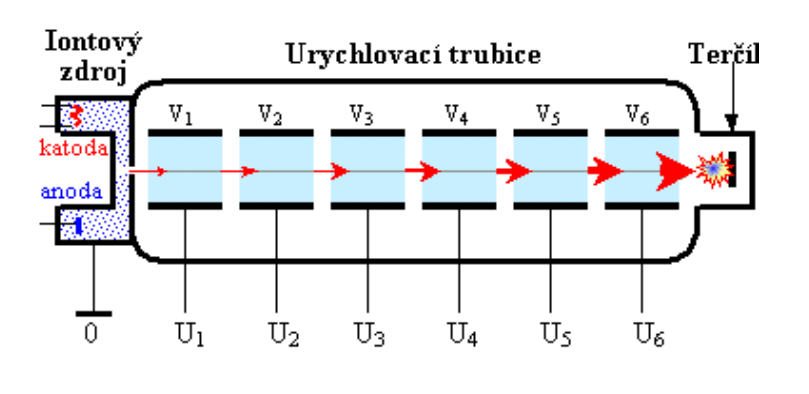
\includegraphics[width=0.7\textwidth]{em2-linearny1.png}
\caption{Schéma elektrostatického lineárneho urýchľovača.}
\label{em2:img:linearny1}
\end{figure}

Existujú dva typy zdroja napätia (ich názov sa potom používa aj pre názov samotného urýchľovača):
\begin{itemize}
\item Cockroft-Waltonov generátor

Jeho základom je násobič napätia. V kaskádovom generátore sa vysoké napätie dosiahne mnohonásobným zvýšením striedavého napätia, získaného transformátorom. Cockroft-Waltonov urýchľovač sa v dnešnej dobe používa v obrích urýchľovačoch ako predstupeň hlavného urýchľovača. Získaná energia je až 4 MeV.

\begin{figure}[h]
\centering
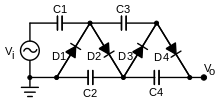
\includegraphics[width=0.5\textwidth]{em2-cockroft.png}
\caption{Schéma dvojstupňového Cockroft-Waltonovho generátoru.}
\label{em2:img:cockroft}
\end{figure}

\item Van der Graafov generátor

Van der Graafov generátor je anglická hudobná skupina hrajúca progresívny rock. Kapela bola založená v roku 1967 v Manchesteri spevákom Peterom Hammillom. Tou sa ale zaoberať nebudeme. Nás totiž zaujíma zdroj vysokého napätia s rovnakým názvom.

Toto zariadenie je založené na známom pokuse z elektrostatiky a v zmenšenom prevedení ho nájdeme v každom fyzikálnom kabinete. Princíp tohto generátoru je v tom, že pokiaľ sa vnútri vodiča nachádza dutina, v ktorej nie sú žiadne makroskopické náboje, zostáva intenzita elektrického poľa v tejto dutine nulová. Pole v dutine je vykompenzované poľom povrchových nábojov. Pomocou pohyblivého pásu z izolujúceho materiálu, ako napr. hodváb či guma, sa prenáša kladný náboj z externého zdroja do vnútra kovovej gule, tam je potom odvedený na jej povrch a pole vnútri ostáva nulové. Vybitá časť pásu sa potom vracia k novému nabitiu. S opakovaným privádzaním náboja do vnútra vodiča môžeme tento
 vodič nabiť teoreticky neobmedzene veľkým nábojom. Obmedzenie potenciálu, dosiahnuteľného na guľách elektrostatického generátoru je dané prierazným napätím obklopujúceho plynu. Preto sa ukázalo účelnejším umiestniť generátor do vzduchotesného obalu, vnútri ktorého sa vytvorí tlak niekoľko atmosfér, čím sa zvyšuje prierazné napätie. Ešte účinnejšie je umiestnenie generátoru v stlačenom plyne s veľkou elektrickou pevnosťou, napr. freón. 

\begin{figure}[h]
\centering
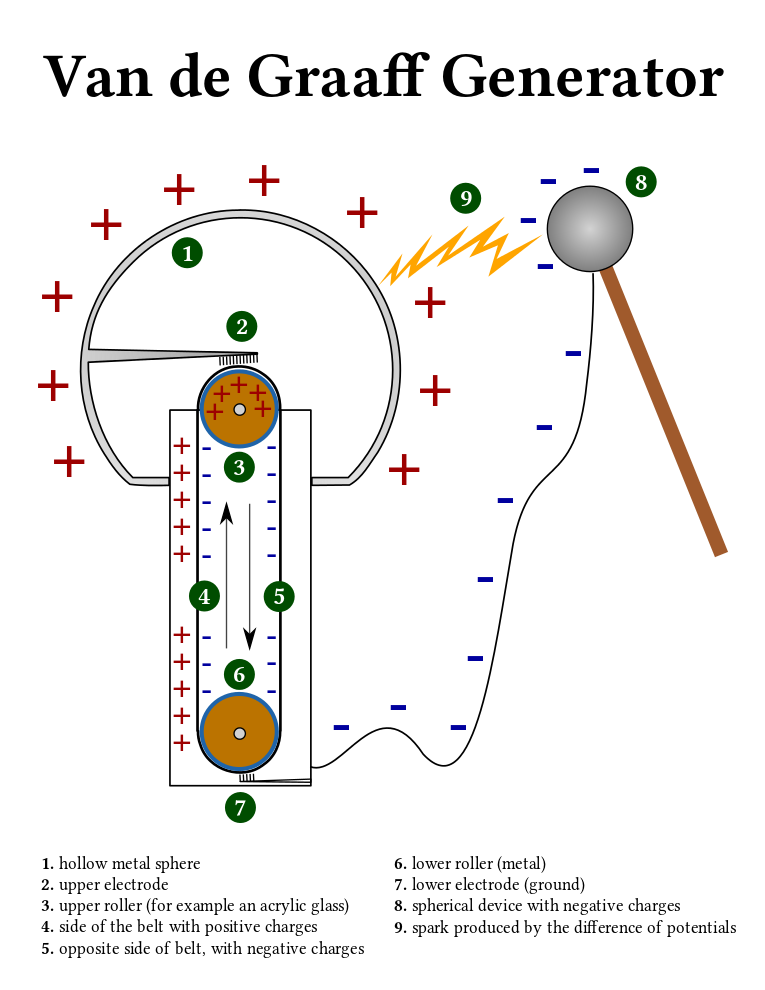
\includegraphics[width=0.5\textwidth]{em2-vandergraf.png}
\caption{Schéma Van der Graafovho generátoru.}
\label{em2:img:vandergraf}
\end{figure}

\end{itemize}

Malý elektrostatický urýchľovač elektrónov mal kedysi doma každý z nás, jedná sa totiž o televíznu CRT (Cathode Ray Tube) obrazovku, v ktorej sa elektróny urýchľujú elektrickým poľom s napätím okolo 16 kV.

\subsection{Vysokofrekvenčné lineárne urýchľovače}

Jedná sa o efektívnejší spôsob urýchľovania nabitých častíc na vysokú energiu bez použitia enormne vysokého napätia. Zo zdroja $Z$ sú častice emitované do urýchľovacieho systému valcových elektród $V_1$, $V_2$, ..., $V_n$, ktoré sú pripojené ku striedavému elektrickému napätiu
\begin{equation}
U(t)=U_0\cos(\omega t)=U_0\cos(2\pi ft)
\end{equation}
s amplitúdou $U_0$ a frekvenciou $f$. K jednému pólu vysokofrekvenčného zdroja elektrického napätia sú pripojené nepárne valce, k druhému pólu párne valce. Ak prejde kladná častica s nábojom $q$ a hmotnosťou $m$ zo zdroja $Z$ vo fáze, kedy prvá valcová elektróda $V_1$ má záporný potenciál $-U_0$, potom získa energiu $E_1=qU_0$ a rýchlosť $v_1=\sqrt{\frac{2qU_0}{m}}$, takže vzdialenosť $l_1$ vnútri valca $V_1$ preletí za čas $t_1=\frac{l_1}{v_1}$. Frekvenciu $f$ striedavého napätia volíme práve tak, aby častica vstúpila do medzery medzi valcami v okamžiku, kedy sa polarity obrátia a valec $V_1$ má kladný potenciál a valec $V_2$ naopak záporný potenciál, potom sa častica znovu urýchli o energiu $qU_0$, čo znamená, že má už energiu $2qU_0$. Pokiaľ chceme docieliť to, aby sa častice pri prechode každou elektródou urýchlila, musí byť synchronizácia medzi frekvenciou $f$, napätím $U$ a dĺžkami elektród $l_k$ volená tak, aby sa obrátila polarita striedavého napätia behom prechodu častíc medzi elektródami. Ako je vidieť na obrázku \ref{em2:img:linearny2}, musí sa dĺžka valcových elektród zvyšovať, ako narastá rýchlosť častíc. K samotnému elektrickému urýchleniu potom dochádza v medzerách medzi elektródami, vnútri valcov prelietajú častice iba vďaka zotrvačnosti.

\begin{figure}[h]
\centering
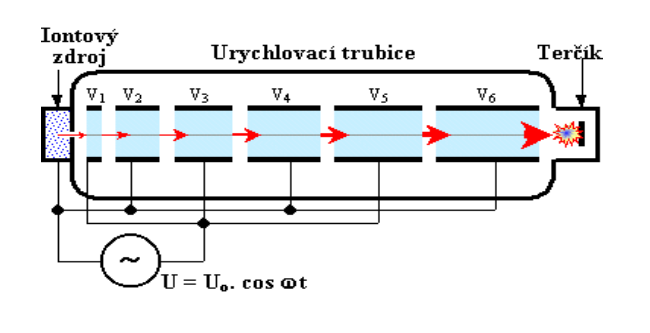
\includegraphics[width=0.7\textwidth]{em2-linearny2.png}
\caption{Schéma vysokofrekvenčného lineárneho urýchľovača.}
\label{em2:img:linearny2}
\end{figure}

Vývojom lineárnych vysokofrekvenčných urýchľovačov sa frekvencia $f$ stále zvyšovala a valcové elektródy nahradili dutinové rezonátory. Tieto lineárne urýchľovače používajú na vytvorenie urýchľujúceho poľa vlnovody, napájané frekvenciou niekoľko GHz z klystronových generátorov.

\begin{itemize}
\item vysokofrekvenčné lineárne urýchľovače s postupnou vlnou

Tieto urýchľovače sa používajú na urýchlenie elektrónov. Urýchľovaciu trubicu tvorí vlnovod, ktorým postupuje elektromagnetická nosná vlna. Po vstreknutí častíc zo zdroja do vlnovodu sa tieto častice stretnú s nosnou vlnou, fázová rýchlosť vlny je menšia než rýchlosť svetla. Pokiaľ budú mať častice v okamžiku stretu zhodnú rýchlosť s elektromagnetickou vlnou, budú si svoju polohu vzhľadom k vlne zachovávať. Tým budú častice trvalo pod vplyvom urýchľujúceho poľa, ako keď morská vlna nesie loďku. Tento vlnovod je v podstate valcovitá trubica, v ktorej sa nachádzajú kruhové clony s otvorom uprostred. Týmito clonami sa zaistí zaťaženie vlnovodu, vďaka nemu potom bude fázová rýchlosť šírenia elektromagnetickej vlny menšia ako rýchlosť svetla.

\begin{figure}[h]
\centering
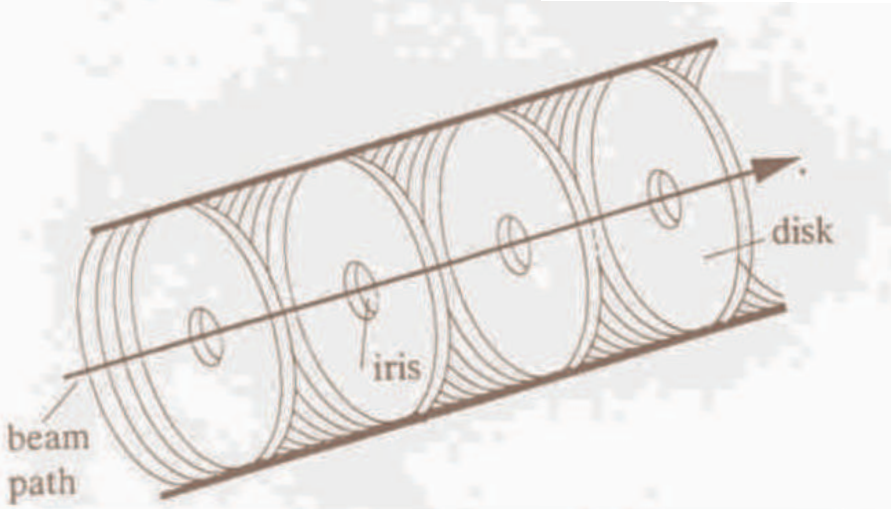
\includegraphics[width=0.7\textwidth]{em2-vlnovod.png}
\caption{Urýchľovacia štruktúra pre elektrónový lineárny urýchľovač s kruhovými clonami.}
\label{em2:img:vlnovod}
\end{figure}

\item vysokofrekvenčné lineárne urýchľovače so stojatou vlnou

Vo vysokofrekvenčnom lineárnom urýchľovači prejde vysokofrekvenčná vlna po urýchľovacej dráhe a na konci sa odrazí naspäť. Vznikne tak stojatá vlna s veľmi veľkým silovým poľom, ktorá silno urýchľuje elektróny do 10 MeV s frekvenciou 100 Hz až 100 kHz. V oboch prípadoch dôjde k veľkému urýchleniu na krátkej dráhe.
\end{itemize} 

\section{Kruhové urýchľovače}

Najväčšie súčasné urýchľovače sú urýchľovače kruhové. Jedná sa o veľmi účinný spôsob, ako urýchľovať nabité častice na vysoké energie ich mnohonásobným urýchlením v elektrickom poli, kam sú opakovane vracané po kruhovej dráhe pôsobením magnetického poľa. Na časticu s nábojom $q$ tu pôsobí ako elektrická urýchľujúca sila $\vec{F}_e=q\vec{E}$, tak aj Lorentzova $\vec{F}_m=q\vec{v}\times\vec{B}$, ktorá pôsobí v magnetickom poli s intenzitou $B$ kolmo na smer pohybu častice s rýchlosťou $v$. Nabitá častica potom vplyvom pôsobenia magnetickej sily koná kruhový pohyb s polomerom $R=\frac{mv}{Bq}$. Pokiaľ je vo vhodných miestach cyklickej dráhy synchrónne použité elektrické pole, častice sú periodicky urýchlené pri každom svojom obehu.

\subsection{Cyklotrón}

Jedná sa o základný typ kruhového urýchľovača. Používa sa na urýchľovanie do energií 15 MeV ťažkých nabitých častíc, napr. protónov alebo deuterónov. 

V cyklotróne sa častice pohybujú vnútri dvoch polkruhových dutých kovových komôr, duantov, označených $D_1$ a $D_2$, umiestnených medzi pólovými nástavcami obrovského magnetu, medzi ktorými sa nachádza urýchľovacia medzera. K duantom je priložené striedavé napätie $U=U_0\cos(2\pi ft)$. Po tom, čo sú častice vstreknuté zo zdroja do stredu urýchľovacej medzery, sú vďaka pôsobeniu elektrickej sily vtiahnuté do jedného z duantov, ktorý má práve opačnú polaritu. Vnútri duantu je potom sila elektrického poľa odtienená silou silného magnetického poľa, vďaka ktorej sa častice pohybuje po polkružnici s polomerom $R=\frac{mv}{Bq}$. Frekvencia obehu častice je konštantná $f=\frac{Bq}{2\pi m}$. Častica sa pohybuje po špirálovej dráhe, kde ju drží časovo nemenné magnetické pole. Aby sme dosiahli synchronizáciu, musí byť frekvencia zdroja zhodná s frekvenciou obehu častice. Keď častica opíše polkružnicu v prvom duante, dorazí opäť do urýchľovacej medzery medzi duantami. Polarita je už opačná, častica je opäť urýchlená elektrickým poľom, čo znamená, že do druhého duantu je vtiahnutá s rýchlosťou $v_2$, ktorá je väčšia než rýchlosť $v_1$, s ktorou bola vtiahnutá do prvého duantu. Pri prechode z jedného duantu do druhého sa častica vždy urýchli a zväčší sa tiež polomer jej dráhy, čo znamená, že častica sa pohybuje po špirále. To sa deje, až pokým častica nevstúpi do poslednej dráhy, ktorá má maximálny polomer. Tu je potom magneticky alebo elektrostaticky vyvedená a narazí na terčík, kde vyvolá požadované procesy. Ak častica dosiahne relativistické rýchlosti, začne jej hmotnosť rásť a doba obehu sa predĺži. Rast hmotnosti v závislosti na rýchlosti je vyjadrený vzťahom $m=\frac{m_0}{\sqrt{1-v^2/c^2}}$. Častica už preto nemôže byť urýchľovaná striedavým napätím s konštantnou frekvenciou, ale urýchlovaciu frekvenciu treba prispôsobiť frekvencii obehu častíc tak, aby s ňou bola stále v rezonancii. Takto modifikovaný cyklotrón sa nazýva fázotron alebo synchrocyklotrón. 

\begin{figure}[h]
\centering
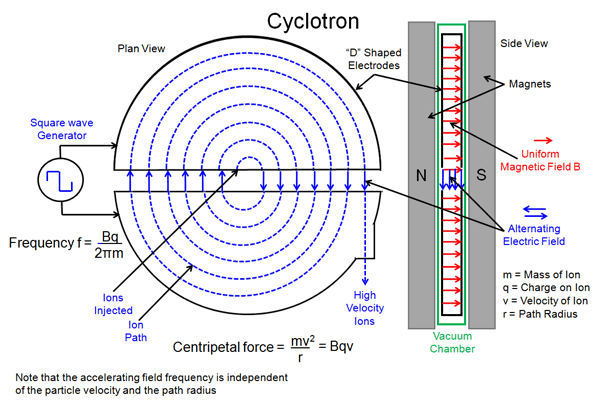
\includegraphics[width=\textwidth]{em2-cyclotron.png}
\caption{Schématické znázornenie cyklotrónu.}
\label{em2:img:cyclotron}
\end{figure}

\subsection{Synchrocyklotrón}

Pre dosiahnutie vyšších energií je nutné kompenzovať vplyv rastu relativistickej hmotnosti s rýchlosťou, čím je spôsobený pokles uhlovej rýchlosti jednotlivých častíc na ich špirálovom pohybe. Vzhľadom k periodicky sa meniacemu urýchľovaciemu elektrickému poľu s konštantnou frekvenciou sa častice spomaľujú. Periodickou zmenou frekvencie možno dosiahnuť synchronizácie s klesajúcou frekvenciou obiehajúcej častice. Fokuzácia je zaistená vhodným priemetom magnetického poľa.

\subsection{Izochrónny relativistický cyklotrón}

Ďalšie odstránenie nežiadúceho rastu hmotnosti sa spraví nárastom magnetickej indukcie s polomerom dráhy. Tým je ale porušená podmienka axiálnej fokuzácie, vďaka ktorej bolo magnetické pole na okraji slabšie, ako uprostred. Pri izochrónnom relativistickom cyklotróne je magnet rozdelený na sektory, magnetické pole je striedavo silné a slabé a prechod medzi sektormi fokusuje zväzok častíc. Frekvencia vysokofrekvenčného generátoru je konštantná.

Tieto cyklotróny sa používajú do energií asi 600 MeV, možno v nich dosiahnuť prúd niekoľko stoviek $\mu$A. Často sú používané ako mezónové továrne, t.j. z terčíku ožiareného urýchlenými protónmi sa získavajú veľmi intenzívne zväzky mezónov $\pi$ či K. Najvýznamnejší izocyklotron je kanadský Triumf urýchľujúci protóny na 520 MeV.

\begin{figure}[h]
\centering
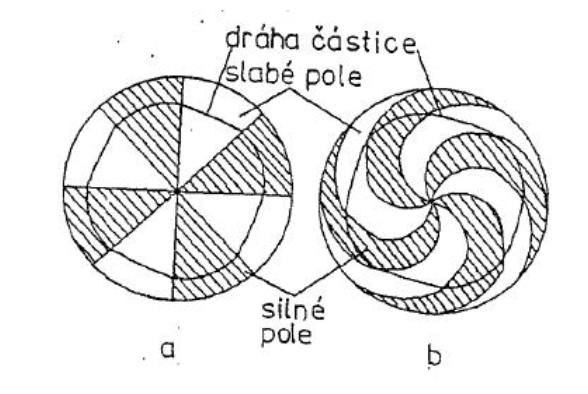
\includegraphics[width=0.6\textwidth]{em2-isocyklo.png}
\caption{Schéma usporiadania magnetického poľa v izochrónnom cyklotróne. Magnet je rozdelený na radiálne (a) alebo špirálne (b) sektory. Vektor magnetickej indukcie $\vec{B}$ smeruje kolmo na obrázok.}
\label{em2:img:isocyklo}
\end{figure}

\subsection{Betatron}

Názov je odvodený od rozpadu beta, ktorého produktom sú práve elektróny. Jedná sa teda o urýchľovač elektrónov. Elektróny, pohybujúce sa na dráhe s nemenným polomerom sú urýchľované silou elektromagnetickej indukcie. Jedná sa v podstate o transformátor, ktorého primárne vinutie je napájané striedavým prúdom a ktorého sekundárnym závitom je vákuová urýchľovacia trubica v tvare prstenca, ktorý je zhotovený z izolujúceho materiálu, ako je napr. sklo, alebo porcelán. Trubica sa nachádza medzi pólovými nástavcami magnetu. Striedavý prúd v primárnej časti urýchľuje elektróny v sekundáre pozdĺž kruhovej dráhy. Už čiastočne urýchlené elektróny sú vo vhodnom okamžiku vstrekované do urýchľovacej trubice elektrónovou tryskou, tvorenou katódou. Ich dráha sa špirálovito zakrivuje, až sa dostanú na kruhovú dráhu, kde sa ich rýchlosť zväčšuje. Na konci urýchľovania sa elektróny pohybujú po špirále z vonkajšej strany, kde narazia na terčík. Elektróny v urýchľovači prebehnú veľmi veľkú dráhu a nepatrné odchýlky znamenajú náraz častice na stenu a stratu energie. Preto je opäť veľmi dôležitá fokuzácia. Tá pôsobí rovno v dvoch smeroch, axiálnom a radiálnom. V axiálnom smere upravujeme magnetické pole pomocou pólových nástavcov magnetu tak, aby na okraji bolo slabšie, než uprostred. V radiálnom sa zaisťuje návrat častíc na stabilnú dráhu.  

Betatrony sa používajú na urýchlenie elektrónov do energií približne 300 MeV\footnote{typicky však urýchľujú elektróny len do energií 20 až 50 MeV}. Častice získajú pri každom obehu približne 100 eV. Betatrony sa v šesťdesiatych až osemdesiatych rokoch používali v rádioterapii, hlavne ako zdroj tvrdého brzdného $\gamma$ žiarenia s energiou do cca 40 MeV.

\begin{figure}[h]
\centering
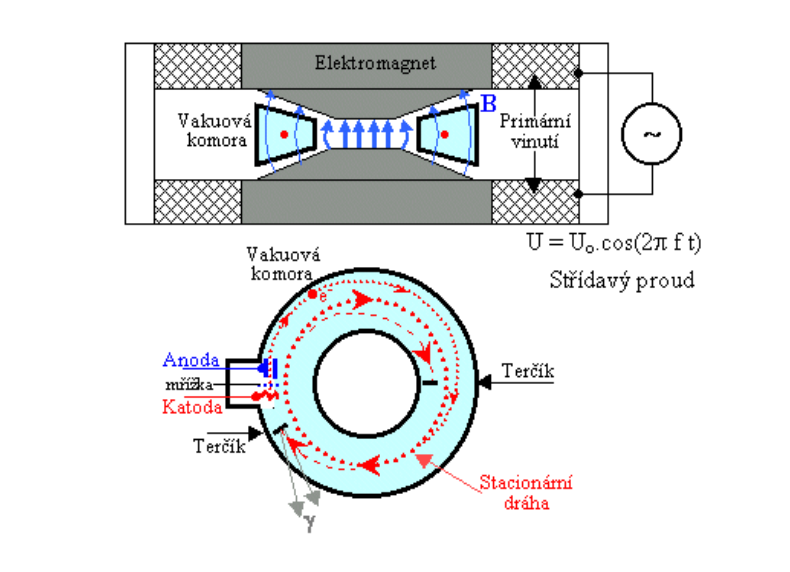
\includegraphics[width=0.6\textwidth]{em2-betatron.png}
\caption{Schématické znázornenie betatronu.}
\label{em2:img:betatron}
\end{figure}


\subsection{Mikrotrón}

Špeciálnym, ale zriedka používaným typom kruhového urýchľovača, je mikrotrón. V magnetickom poli medzi pólovými nástavcami silného elektromagnetu je umiestnená plochá valcová komora s vysokým vákuom, podobne ako pri cyklotróne, avšak miesto duantov je pri okraji komory umiestnený elektrický urýchľovací systém - dutinový rezonátor (napájaný vysokofrekvenčným napätím). Elektróny prelietavajú mnohokrát týmto rezonátorom, kam sú po kruhovej dráhe vracané magnetickým poľom, pričom pri každom prelete sú urýchľované na väčšie a väčšie energie. Vzhľadom ku zvýšenej kinetickej energii je polomer dráhy elektrónu po každom prelete rezonátoru väčší a väčší. Aby elektrón prišiel medzi elektródy rezonátoru v správnej fáze periódy vysokofrekvenčného napätia a mohol byť znovu urýchlený, je treba splniť podmienky rezonancie
\begin{equation}
\omega_c=\dfrac{qBc^2}{mc^2}=\dfrac{qBc^2}{E_k+m_0c^2}.
\end{equation}

Perióda obehu je potom
\begin{equation}
T=\dfrac{2\pi}{\omega_c}=\dfrac{2\pi m_0}{Bq}\left(1+\dfrac{E_k}{m_0c^2}\right)
\end{equation}
a pre polomery dráh platí vzťah
\begin{equation}
R=\dfrac{p}{Bq}=\dfrac{1}{Bqc}\sqrt{E_k(E_k+2m_0c^2)}.
\end{equation}

V mikrotrónoch každé urýchlenie dodá elektrónu energiu $m_0c^2$, ako je zrejmé z tabuľky \ref{em2:tab:mikro}.

\begin{table}[h]
\centering
\begin{tabular}{|l|c|c|c|}
\hline
Urýchlenie & Energia & Doba obehu & Polomer \\ \hline \hline
Prvé & $E_k=m_0c^2$ & $T_1=\dfrac{2\pi m_0}{Bq}\left(1+1\right)=2T_0$ & $R_1=\dfrac{m_0c^2}{Bqc}\sqrt{3}$ \\ \hline
Druhé & $E_k=2m_0c^2$ & $T_2=\dfrac{2\pi m_0}{Bq}\left(1+2\right)=3T_0$ & $R_2=\dfrac{m_0c^2}{Bqc}\sqrt{8}$ \\ \hline
\vdots & \vdots & \vdots & \vdots \\ \hline
$k$-te & $E_k=km_0c^2$ & $T_k=\dfrac{2\pi m_0}{Bq}\left(1+k\right)=(1+k)T_0$ & $R_k=\dfrac{m_0c^2}{Bqc}\sqrt{k(k+2)}$ \\ \hline
\end{tabular}
\caption{Energia, doba obehu a polomer kruhovej trajektórie urýchľovanej častice v mikrotróne.}
\label{em2:tab:mikro}
\end{table}

Frekvencie vysokofrekvenčného generátoru sa volia tak, aby $\tau_{gen}=T_0$. Doba obehu je potom vždy celým násobkom periódy $\tau_{gen}$, vďaka čomu bude elektrón prichádzať do vysokofrekvenčného poľa generátoru vždy v správnej fáze a bude poľom urýchlený.

Elektróny na urýchlenie sa vstrekujú elektrónovým delom, prípadne sa získajú emisiou zo stien rezonátoru. Mikrotróny sa občas používajú na urýchľovanie elektrónov na energiu niekoľko MeV, ich prednosťou je však dosiahnutie vysokých intenzít toku urýchlených elektrónov vo zväzku. Z jednotlivých dráh možno vyextrahovať monoenergetické zväzky elektrónov, z menších dráh nižšie energie, z dráhy s najväčším polomerom pri okraji urýchľovacej komory potom elektróny s maximálnou energiou.

Zvláštnym typom mikrotrónu je tzv. \textit{race-track mikrotron}, v ktorom je magnet rozdelený na dva sektory a medzi nimi je umiestnený lineárny urýchľovač. Príkladom je urýchľovač MAMI v Nemecku, ktorý urýchľuje na 1580 MeV. 

\begin{figure}[h]
\centering
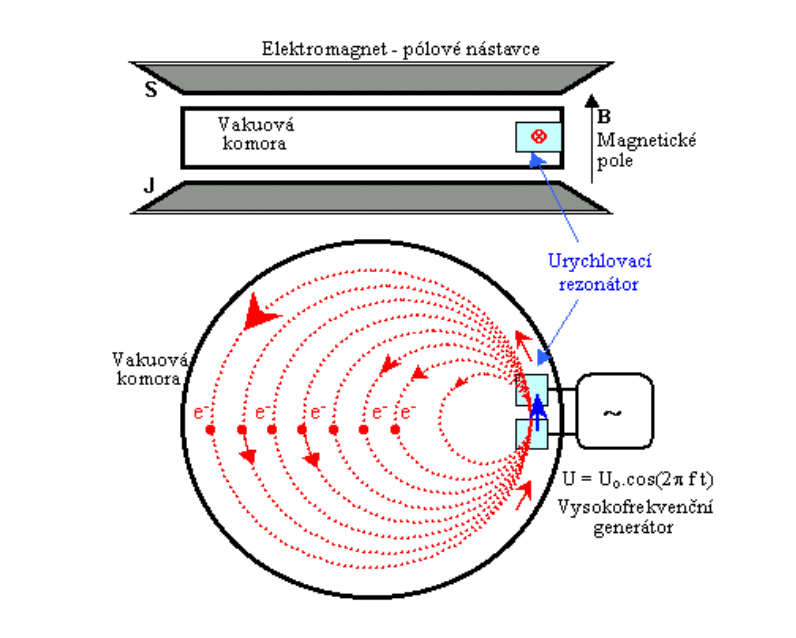
\includegraphics[width=0.6\textwidth]{em2-mikrotron.png}
\caption{Schématické znázornenie mikrotronu.}
\label{em2:img:mikrotron}
\end{figure}

\subsection{Synchrotrón}

Veľké súčasné urýchľovače zvané synchrotróny používajú premenné magnetické pole tak, aby polomer trajektórie zostával nemenný aj pri náraste relativistickej hmotnosti. Rýchlosť je potom takmer rovná rýchlosti svetla. Pokiaľ chceme častice urýchliť na veľmi vysoké energie, vychádza v špirálovom urýchľovači veľký polomer. Preto sa častice v synchrotróne nepohybujú po špirále, ale po kruhovej dráhe vnútri trubice, z ktorej bol vyčerpaný vzduch. Z praktického hľadiska je špirálovitý spôsob urýchlenia na vysoké energie nepoužiteľný. Vákuový priestor aj elektromagnety by dosahovali enormných rozmerov. Muselo teda dôjsť k modifikácii na urýchľovač s pevnou kruhovou dráhou. To umožňuje budovať urýchľovače tvaru prstenca kolosálnych rozmerov, pozdĺž neho sú rozmiestnené magnety. Urýchľovacia komora pritom musí byť umiestnená s milimetrovou presnosťou.

\begin{figure}[h]
\centering
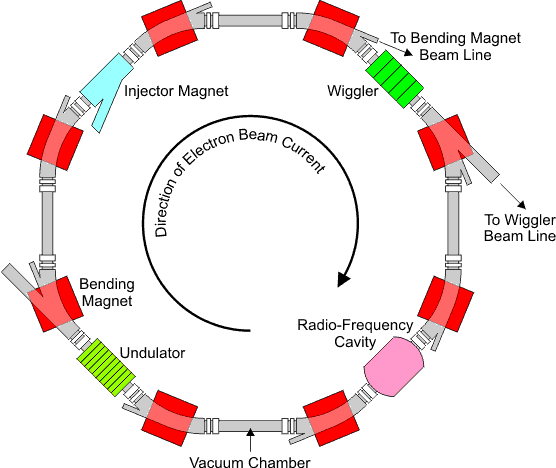
\includegraphics[width=0.6\textwidth]{em2-synchrotron.png}
\caption{Schématické znázornenie synchrotrónu.}
\label{em2:img:synchrotron}
\end{figure}

\begin{itemize}
\item Elektrónový synchrotrón

Používa sa na urýchlenie elektrónov, ktoré sa pohybujú po dráhe s nemenným polomerom. Frekvencia urýchľovacieho napätia je konštantná, naopak magnetická indukcia v priebehu urýchlenia rastie. Toto zariadenie pracuje v počiatočnej fáze rovnako ako betatron (do energie približne 2 MeV). Potom dôjde ku splneniu podmienky pre synchrotrónny režim, urýchľovanie prechádza na pulzný režim. Fokuzácia aj aplikácia je podobná ako pri betatrone.

\item Protónový synchrotrón (Synchrofázotron)

Ak sa v synchrotróne mení aj frekvencia urýchľovacieho napätia, vznikne synchrofázotron. Behom urýchľovania na dráhe s konštantným polomerom rastie teda magnetická indukcia aj frekvencia napätia. Urýchľovacia trubica je vákuová a má väčšinou priemer 3 až 8 cm, tvorí kruh s priemerom stoviek metrov až niekoľko kilometrov. Okolo trubice sú rozmiestnené elektromagnety, majúce tvar kruhového výseku, týchto segmentov býva stovky kusov. Okolo kruhovej dráhy sú na vhodných miestach tiež urýchľovacie elektródy, ktoré sú napájané striedavým vysokým napätím. Frekvencia tohto napätia je synchrónne zvyšovaná, pretože je dôležité, aby častice medzi elektródy prišli práve v tom okamžiku, kedy polarita zaistí ďalšie a ďalšie urýchlenie. Častice, ktoré sú v synchrotróne, sú už predom čiastočne urýchlené v lineárnom urýchľovači na energie približne 20 až 100 MeV. S týmito energiami vstupujú častice z injektoru do urýchľovacej trubice v pravidelných dávkach. Behom urýchľovacieho cyklu, ktorý trvá asi 4 sekundy, vykoná častica až niekoľko miliónov obehov a urýchli sa až na niekoľko TeV. Tento cyklus sa behom minúty niekoľkokrát zopakuje, po jeho skončení dopadnú častice podľa potreby na vonkajší alebo vnútorný terčík. Pokiaľ sa jedná o protichodný zväzok, častice sú zavedené do akumulačného prstenca. Pri náraze na terčík potom vznikne množstvo rôznych druhov častíc, tie potom môžeme odseparovať pomocou magnetických a elektrických polí, fokuzáciou sformovať zväzok a ten potom môže naraziť na ďalší terčík. V takom prípade sa jedná o sekundárne zväzky.

Fokuzácia je dôležitá už pri prechode urýchľovacou trubicou. Častice totiž po vstreknutí konajú radiálne a vertikálne kmity okolo svojej základnej dráhy a tiež sa rozbiehajú zo zväzku do všetkých strán, pretože sa vďaka súhlasnému náboju odpudzujú. Pomocou silnej magnetickej fokuzácie dôjde ku sformovaniu častíc do úzkeho intenzívneho zväzku. Podstata fokuzácie spočíva vo vhodne zostavených segmentoch elektromagnetu, ktoré majú striedavo kladný a záporný gradient intenzity magnetického poľa, čo potom vedie k dvojitej fokuzácii v radiálnom a vertikálnom smere striedavo.
 
\end{itemize}


\subsection{Synchrotrónové žiarenie}

Celkom špeciálny spôsob využitia sekundárneho žiarenia z urýchľovačov spočíva vo využití synchrotrónového žiarenia. Je to elektromagnetické žiarenie, ktoré vyžaruje nabitá častica pri pohybe po zakrivenej dráhe. Z hľadiska funkcie kruhových urýchľovačov je to jav parazitný a nepriaznivý, ktorý bráni dosahovať vysoké energie, obzvlášť pri elektrónoch. Avšak UV a RTG zložka synchrotrónového žiarenia môže byť využitá v niektorých aplikáciach, napr. pri analýze materiálov alebo v biológii či v medicínskej diagnostike.

Ako je známe zo zákonov elektrodynamiky, častica s pokojovou hmotnosťou $m_0$, nábojom $q$, pohybujúca sa s kinetickou energiou $E$ po dráhe s polomerom $R$ vyžaruje elektromagnetické vlny výkonom
\begin{equation}
P=\dfrac{2}{3}\dfrac{q^2c}{R^2}\left(\dfrac{E}{m_0c^2}\right)^4.
\end{equation}

Z tejto rovnice vidíme, že vyžarovanie je podstatné iba pre ľahké nabité častice (elektróny či pozitróny) pohybujúce sa s vysokou energiou, t.j. relativistickou rýchlosťou po silne zakrivenej dráhe. Pri pomalom pohybe sa obiehajúce častice javia ako oscilujúci elektrický dipól vyžarujúci slabé monochromatické žiarenie (s frekvenciou danou periódou obehu) prakticky do všetkých smerov.

Pri pohybe častice relativistickou rýchlosťou je však elektromagnetické žiarenie vysielané v úzkom kuželi, ktoré osou je dotyčnica k orbite v danom bode. Uhol otvorenia tohto kužeľa je približne rovný $\frac{m_0c^2}{E}$. Vonkajší pozorovateľ navyše bude schopný detekovať žiarenie iba počas doby, kedy tento kužeľ pretína jeho stanovisko (\quotedblbase majákový efekt\textquotedblright ). Pri pohybe častice po kruhovej dráhe bude teda pevný pozorovateľ registrovať pulzy žiarenia, ktorých frekvencia je daná dobou obehu častice $T=\frac{L}{c}$, kde $L$ je dĺžka orbity.

Spektrum vlastného synchrotrónového žiareniasa skladá z radu harmonických zložiek, ktoré sú v dôsledku priebežného pohybu po orbite natoľko rozmazané, že sa výsledné spektrum javí ako spojité.

\section{Fokuzácia a fázovanie}

\subsection{Slabá fokuzácia}

Cieľom fokuzácie je návrat urýchľovanej častice na stabilnú orbitu polomeru $R$. Pri fokuzácii je nutné pôsobiť na časticu v dvoch smeroch - \textit{axiálnom} (axiálnu fokuzáciu dosiahneme vhodným tvarom pólových nástavcov - na okraj je magnetické pole slabšie než v strede) a \textit{radiálnom} (radiálna fokuzácia vyžaduje, aby magnetické pole zoslabovalo od stredu k okrajom pomalšie, než $\frac{1}{r}$), keďže nabitá častica pri urýchľovaní vykonáva okolo stabilnej orbity tzv. \textit{betatrónové kmity} - jednak axiálne a tiež radiálne.

Prakticky možno fokuzáciu zaistiť vhodným tvarom pólových nástavcov magnetu. V tomto spôsobe sa volí závislosť magnetickej indukcie na polomere $r$ v tvare
\begin{equation}
B(r)=B(R)\left(\dfrac{r}{R}\right)^{-n},
\end{equation}
kde $0<n<1$ je index poľa. Vzhľadom k jeho malej hodnote sú magnetické fokusačné sily slabé, priečne rozmery zväzku sú relatívne veľké a tým pádom rozmery urýchľovacích komôr veľké.

\subsection{Silná fokuzácia}

Pri veľkých komorách s polomerom $R$, ktorý na dosiahnutie vysokých energií rádovo stoviek GeV musí dosahovať niekoľko kilometrov, je potrebné, aby prierez urýchľovacej trubice bol čo najmenší - aby bolo možné dosiahnuť potrebného vákua a aby náklady na výrobu elektromagnetov, ako aj nároky na ich elektrický príkon, neboli extrémne vysoké.

Častice po vstreku do urýchľovacej trubice konajú radiálne a vertikálne kmity okolo svojej základnej kruhovej dráhy. Okrem toho majú častice v zväzku tendenciu rozbiehať sa do všetkých strán, pretože sú súhlasne nabité a odpudzujú sa. Ak nemá dôjsť k dopadu častice na stenu trubice, je treba udržať urýchľované častice na ich orbite s vysokou presnosťou, takže je treba udržať amplitúdu radiálnych a vertikálnych kmitov čo najnižšiu, rovnako ako rozptyl častíc.

Inými slovami, je treba spraviť silnú fokuzáciu, pri ktorej sa zhluk vstreknutých častíc behom urýchľovania koncentruje a formuje do intenzívneho úzkeho zväzku prudko letiacich častíc. Táto silný magnetická fokuzácia je realizovaná tak, že elektromagnet synchrotrónu je zostavený z veľkého počtu vhodne tvarovaných segmentov, ktoré majú striedavo kladný a záporný gradient intenzity magnetického poľa. Tieto gradienty magnetického poľa pôsobia v radiálnom a vertikálnom smere striedavo ako spojne a rozptylné magnetické šošovky, ktoré v konečnom dôsledku vedú k dvojitej fokuzácii zväzku v oboch smeroch.

Silná fokuzácia sa používa v protónových synchrotrónoch. Magnet je rozdelený na párny počet sektorov - magnety tak budia okrem homogénneho poľa aj nehomogénne pole s veľkým indexom $\sim 300$. Indexy poľa a gradienty sú striedavo kladné a záporné, striedavo sa vykonáva radiálna fokuzácia a axiálna defokuzácia a naopak.

\subsection{Magnety v urýchľovačoch}

Častice v urýchľovačoch musia byť usmerňované silou takým spôsobom, aby sa pohybovali po približne kruhovej dráhe. To môžeme dosiahnuť použitím dipólového elektrostatického alebo dipólového magnetického poľa. Väčšina urýchľovačov však urýchľuje relativistické nabité častice, takže je praktickejšie používať dipólové magnety. 

Dipólové magnety sami o sebe ale obstarávajú iba slabú fokuzáciu a urýchľovače používajúce iba tento typ magnetov by mali veľmi veľké zväzky. Preto sú dipólové magnety dopĺňané kvadrupólovými a sextupólovými magnetmi, ktoré zabezpečujú silnú fokuzáciu. 

Dipólové magnety vytvárajú homogénne magnetické pole. Častice sa v ňom pohybujú po kruhovej trajektórii kolmo na smer magnetickej indukcie. V urýchľovačoch sa dipólové magnety okrem samotného ohýbania trajektórie používajú na injekciu a ejekciu častíc z a do urýchľovača, korekciu orbít a produkciu synchrotrónového žiarenia.

Kvadrupólové magnety môžu byť typ F a typu D. F kvadrupóly fokusujú zväzok horizontálne, no zároveň ho vertikálne defokusujú. D kvadrupóly fungujú presne naopak. Zákony elektromagnetizmu totiž neumožňujú, aby kvadrupól dokázal fokusovať v oboch smeroch súčasne. Ak sú F a D kvadrupóly umiestnené striedavo za sebou, ich polia sa vzájomne vyrušia. Ak je však medzi nimi medzera (s vhodnou veľkosťou), výsledným efektom bude fokuzácia vo vertikálnom aj horizontálnom smere.

Sextupólové magnety majú ohniskovú vzdialenosť nepriamo úmernú vzdialenosti od stredu magnetu. Sila, ktorá na častice pôsobí je teda úmerná vzdialenosti od osi zväzku. Pokiaľ sextupólový magnet uložíme na miesto, v ktorom častice v zväzku sú usporiadané podľa ich energie, sextupól bude pôsobiť ako sila, ktorá fokusuje častice všetkých energií do jedného bodu. To vyruší tendenciu kvadrupólových magnetov rozbiehať zväzok.

\begin{figure}[h]
\centering
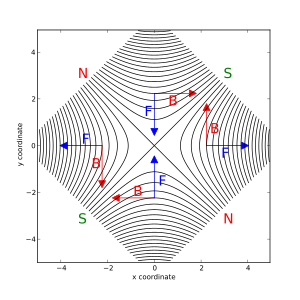
\includegraphics[width=0.48\textwidth]{em2-4pol.png}
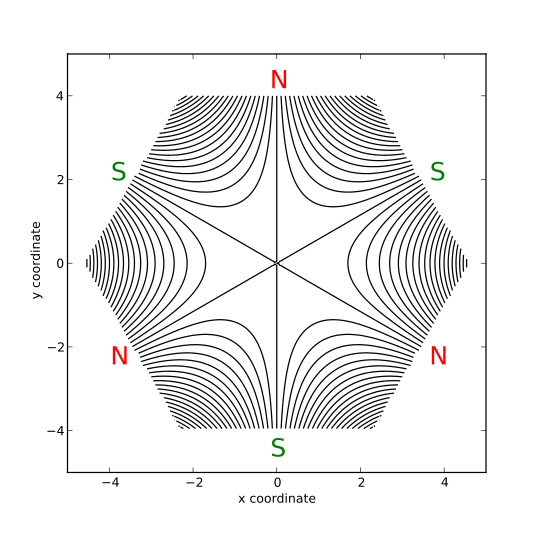
\includegraphics[width=0.48\textwidth]{em2-6pol.png}
\caption{Magnetické pole ideálneho kvadrupólu (naľavo) a sextupólu (napravo).}
\end{figure}

\subsection{Fázovanie}

Fázová stabilita zaistí oneskoreným či zrýchleným časticiam návrat do rezonancie s vysokofrekvenčným poľom.

\begin{enumerate}
\item Častica v rezonancii s vysokofrekvenčným poľom prilieta v čase $t_0$, na štrbine je napätie $U=0$. Pre $t_0=0,2\pi,4\pi,\ldots$ sa ich energia nezmení.
\item Častica príde skôr, t.j. $t_1<t_0$, kedy $U>0$. Zväčší sa hmotnosť častice, tým pádom $\omega<\omega_c$ a $T>T_c$. Častica sa zjavne oneskoruje a postupne sa dostáva na rovnovážnu dráhu.
\item Častica sa oneskoruje, t.j. $t_2>t_0$, kedy $U<0$. Zmenšuje sa hmotnosť častice, tým pádom $\omega>\omega_c$ a $T<T_c$. Častica sa urýchľuje a postupne sa dostáva na rovnobežnú dráhu.
\end{enumerate}

Pre rovnovážne hodnoty platia vzťahy (pri konštantnom $R$ a $B$):
\begin{subequations}
\begin{equation}
\omega_c=\dfrac{Bq}{m}
\end{equation}
\begin{equation}
T_c=\dfrac{2\pi m}{Bq}
\end{equation}
\end{subequations}

Aby sme to zhrnuli, fáza, frekvencia, energia a polomer dráhy častice oscilujú okolo rovnovážnej polohy odpovedajúcej rezonancii pohybu častice s urýchľujúcim poľom. Toto fázovanie je samočinné. Princíp fázovej stability možno využiť aj na urýchľovanie častíc (v synchrocyklotróne či elektrónovom synchrotróne).

\section{Laserové plazmové urýchľovače}

Pri prechode intenzívneho svetelného lúča z laseru plynným prostredím dochádza k ionizácii plynu, vzniká plazma. Ak ožiarime plynné prostredie veľmi intenzívnym krátkym pulzom laserového svetla, vzniká v prostredí plazmová stopa, ktorá za sebou strháva uvoľnené elektróny. Tie sa tu pohybujú v prostredí kladných iónov pri pôsobení Coulombickej sily, pričom môže dochádzať k periodickému vychyľovaniu súboru elektrónov voči súboru iónov (ktoré sa vďaka svojej podstatne väčšej hmotnosti takmer nepohybujú) - k osciláciám elektrónov v Coulombickom poli, sprevádzaným periodicky premenným elektrickým poľom. Vzniká akási stopa vlniacej sa koncentrácie elektrónov a intenzity elektrického poľa - plazmová vlna, podobná vlniacej sa stope alebo brázde, ktoré za sebou zanecháva loď rýchlo plávajúca po vodnej hladine.

Frekvencia oscilácii elektrónov v plazmovej vlne je
\begin{equation}
\omega_p=\dfrac{r_pq^2}{\epsilon_0m_e},
\end{equation}
kde $m_e$ je hmotnosť elektrónu, $q$ jeho náboj a $r_p$ hustota plazmy. Pri osciláciách elektrónov v plazmovej vlne vzniká striedavé elektrické pole s amplitúdou intenzity
\begin{equation}
E_{max}=\dfrac{m_e\omega_pc}{q}
\end{equation}

Pre hustoty $r_p\gg 10^{18}$ častíc/cm$^3$ dosahuje urýchľujúci gradient hodnoty $E\gg 1$ GeV/cm, čo je o dva až tri rády viac, než v lineárnych urýchľovačoch.

Pozdĺžna zložka oscilujúceho elektrického poľa v tejto plazmovej vlne môže za určitých okolností urýchľovať elektróny, ktoré sú nesené na vlne elektrického poľa.

Pri použití laseru s pikosekundovými pulzmi s vysokou intenzitou vzniká veľmi intenzívne pozdĺžne urýchľovacie pole, ktoré môže elektróny urýchliť na energiu asi 50 MeV. Pokusné urýchľovače založené na tomto princípe dostali názov LWFA (\textit{Laser Waked Field Accelerator}). Ich výhodou sú malé rozmery, navyše rýchly pokrok laserovej techniky sľubuje možnosti efektívneho urýchľovania riadeného niekoľkými sekvenčnými laserovými pulzmi.

\begin{figure}[h]
\centering
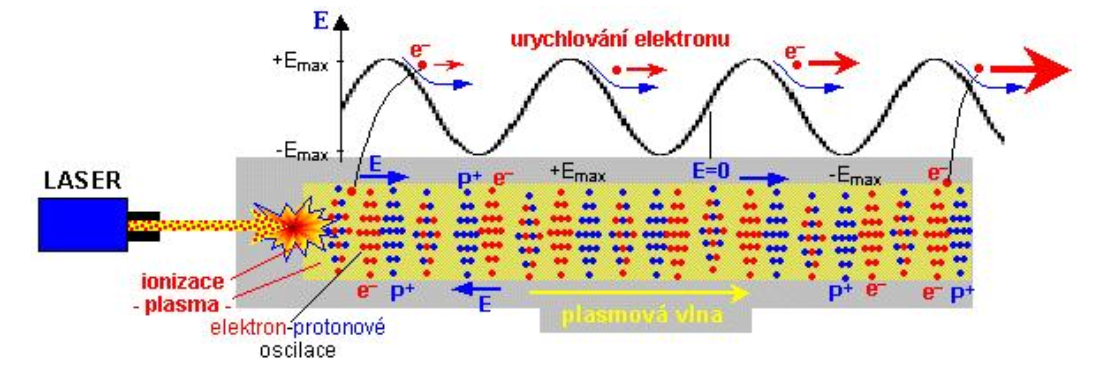
\includegraphics[width=0.8\textwidth]{em2-laser.png}
\caption{Schéma laserového plazmového urýchľovača.}
\label{em2:img:laser}
\end{figure}

\section{Najvýznamnejšie urýchľovače}

\subsection{LHC}

Zatiaľ najväčší urýchľovač bol vybudovaný v európskom centre pre jadrový výskum (CERN) na švajčiarsko-francúzskom pomedzí pod názvom \textbf{Veľký Hadrónový Zrážač} (LHC).

LHC je synchrotrón, ktorého prstenec sa nachádza v tuneli po predchádzajúcom elektrónovom urýchľovači LEP asi 50 až 150 metrov pod zemou a jeho obvod je 27 km.

Keďže LHC je synchrotrón, potrebuje na svoju činnosť už predurýchlené častice\footnote{približne na 0,45 TeV} - sú dokonca štvorstupňovo predurýchlené. Protóny, získané ionizáciou vodíku, sú najskôr urýchlené v lineárnom urýchľovači LINAC na energiu 50 MeV, odtiaľ sú vedené do kruhového urýchľovača Proton Synchrotron Booster, kde získajú energiu 1,4 GeV. Potom sú nasmerované do prstenca protónového synchrotrónu PS s výstupnou energiou 25 GeV a nakoniec do ďalšieho synchrotrónu SOS (Super Proton Synchrotron), ktorý im udelí energiu 0,45 TeV. S touto východzou energiou sú injektované k finálnemu urýchleniu do prstenca hlavného urýchľovača LHC, kde sú behom miliónu obehov (a približne dvadsiatich minút) urýchlené na 7 TeV.

Vzhľadom k tomu, že synchrotrón pracuje v pulznom režime, urýchľujú sa protóny v skupinách či zhlukoch. Protóny sa urýchľujú v dvoch trubiciach v opačných smeroch. Okrem protónov urýchľuje LHC aj ťažšie jadrá, predovšetkým jadrá olova alebo po novom aj xénia. 

Po obvode LHC sú štyri miesta, kde sa trubice prepájajú a protismerné zväzky častíc sa krížia - tu prebiehajú zrážky. Tieto miesta sú obklopené veľkými a zložitými detekčnými systémami, pomocou ktorých je pripravených šesť experimentov. Keďže každý z týchto experimentov sa sústredí na odlišnú problematiku, medzi jednotlivými experimentami sú rozdiely v metóde detekcie, štruktúre detektoru a získavaní dát. Niekoľko experimentov si v ďalšom texte popíšeme detajlnejšie.

\begin{figure}[h]
\centering
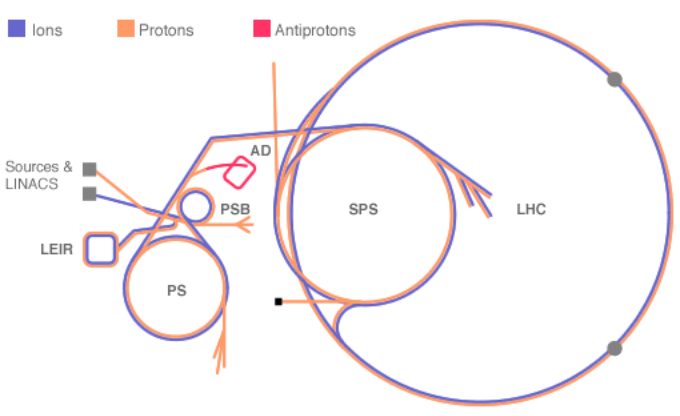
\includegraphics[width=0.8\textwidth]{em2-lhc.png}
\caption{Schématický diagram urýchľovacieho komplexu v CERNe.}
\label{em2:img:lhc}
\end{figure}

\paragraph{ATLAS (A Toroidal LHC Apparatus)}

ATLAS je naväčším detekčným systémom, hlavným nosným programom LHC\footnote{Túto vetu môžte použiť iba v prípade, že v miestnosti nie je nikto z ALICE}. Má za úlohu komplexne merať a analyzovať častice vznikajúce pri zrážkach protónov s energiou 14 TeV. Detekčný systém ATLAS má valcové koaxiálne usporiadanie, pričom je najzložitejším a najnákladnejším detekčným zariadením v doterajšej histórii.

Vnútorná časť detektoru, ktorá zaznamenáva dráhy nabitých častíc vylietavajúcich z miesta zrážky, sa skladá z troch vrstiev dráhový detektorov: najnižšie sú polovodičové pixelové detektory, potom stripové detektory a detektory prechodového žiarenia. Celý systém je umiestnený v silnom pozdĺžnom magnetickom poli supravodivého solenoidálneho elektromagnetu - zo zakrivenia dráh častíc v magnetickom poli možno určiť náboj a hybnosť častíc.

Ďalšiu vrstvu detekčného systému tvorí spektrometer, ktorého úlohou je absorbovať energiu vylietavajúcich častíc a kvantifikovať ju pomocou výstupných elektrických impulzov.

Poslednou vrstvou, vonkajšou, je miónový spektrometer, určený na detekciu vysokoenergetických miónov, ktoré sú schopné prejsť vrstvou spektrometru. Analýzou dráh miónov, zakrivených silným toroidálnym magentickým poľom, možno určiť ich hybnosti a znamienka elektrických nábojov. K detekcii dráh miónov sa používajú driftové trubicové a mnohokáblové ionizačné komory.

\paragraph{CMS (Compact Muon Solenoid)}
Detektor CMS je optimalizovaný na detailnú analýzu miónov. Mal by spolupracovať so systémom ATLAS kvôli komplexnej analýze vysokoenergetických interakcií. Jeho štruktúra je podobná ako v ATLASe. Na analýzu trajektórii rýchlych miónov je súčasťou detekčného systému veľký elektromagnet valcového tvaru (solenoid) vytvárajúci magnetické pole s veľkosťou 4 T. Na deteknčých systémoch ATLAS a CMS sa očakáva objav nových častíc.

\paragraph{ALICE (A Large Ion Collider Experiment)}

ALICE je ďalším experimentálnym systémom, ktorého úlohou je štúdium zrážok jadier (ťakžých iónov), predovšetkým olova (xénia), s ťažiskovou energiou až 5 GeV/nukleón a skúmanie vlastností vznikajúcej kvark-gluónovej plazmy.

ALICE má valcové koaxiálne usporiadanie veľkého počtu detektorov, určených k registrácii a rekonštrukcii parametrov predovšetkým nabitých častíc vznikajúcich pri zrážkach jadier. Mal by slúžiť na štúdium extrémnych stavov hmoty pri podobných podmienkach, aké boli vo vesmíre na počiatku hadrónovej éry, t.j. v prvých mikrosekundách existencie vesmíru.

\paragraph{TOTEM (Total Cross Section, Elastic Scattering and Diffraction Dissociation)}

TOTEM má slúžiť k presnému meraniu efektívnych rozmerov protónu - účinných prierezov - pre rôzne druhy interakcií a tiež na kalibračné meranie vlastností LHC ako je napr. luminozita (účinnosť produkcie zrážok v urýchľovači). Tvorený je ôsmymi detektormi umiestnenými blízko zrážajúcich sa zväzkov v detektore CMS.

\paragraph{LHCb (Large Hadron Collider beauty)}

LHCb má za úlohu študovať narušenie CP-symetrie pri rozpadoch B-mezónov obsahujúcich ťažký bottom kvark. Pri vysokoenergetických zrážkach protónov v LHC vzniká mimo iné aj veľký počet párov $b-\bar{b}$ a ich hadronizáciou B-mezóny a baryóny. Spôsob rozpadu táchto častíc je citlivý na narušenie CP-symetrie\footnote{teda na to, či sa hmota chová odlišne ako antihmota}.

Častice sú najskôr lokalizované detektorom VELO (VErtex LOcator) umiestneným blízko miesta zrážky. Identifikácia častíc pre prechodom a po prechode dipólovým magnetickým poľom je prevádzaná pomocou dvoch prstencových zobrazovacích Čerenkovových detektorov RICH (Ring Imaging Cherenkov detectors). Komora RICH1 sa nachádza hneď za detektorom VELO, za magnetom je detektor stôp častíc, nasleduje komora RICH2 na identifikáciu častíc s veľkou hybnosťou. Ďalej sú zaradené elektromagnetické a hadrónové kalorimetre na meranie energie častíc. Nakoniec sú umiestnené miónové komory.

Výsledky z LHCb môžu byť zaujímavé z hľadiska vzniku nerovnováhy medzi hmotou a antihmotou (baryónová asymetria) v počiatočných fázach vývoja vesmíru.

\subsection{SPS}

Super Proton Synchrotron je urýchľovač častíc pracujúci v CERNe. Pôvodne mal urýchľovať na energie 300 GeV, následne sa dosiahla energia 400 GeV.

Medzi rokmi 1981 a 1984 slúžil ako protón-antiprotónový zrážač (označenie $Sp\bar{p}S$) a ním urýchlené zväzky častíc poskytovali dáta k experimentom UA1 a UA2, ktoré vyústili k objavu W a Z bozónov. V súčasnej dobe je SPS používaný ako koncový predurýchľovač protónových zväzkov s vysokou intenzitou pred ich vstupom do LHC.

\subsection{Tevatron}

Tevatron je kruhový urýchľovač pracujúci vo Fermilabe. Je schopný urýchľovať častice na energie 1 TeV (odtiaľ pochádza jeho názov). Je to synchrotrón a urýchľuje protóny a antiprotóny.

K urýchľovaniu dochádza v niekoľkých etapách. Tou prvou je Cockcroft-Waltonov predurýchľovač urýchľujúci na 750 keV, v ktorom sa ionizuje plynný vodík a urýchľujú záporné ióny použitím kladného napätia. Ióny následne cestujú 150 metrov dlhým lineárnym urýchľovačom, ktorý používa oscilujúce elektrické pole na urýchlenie iónov na energiu 400 MeV. Ióny následne prechádzajú fóliou uhlíku, kde sa zbavia elektrónov. Protóny potom pokračujú do Boosteru.

Booster je malý kruhový urýchľovač, ktorý udelí protónom energiu 8 GeV. Tie následne pokračujú do hlavného injektoru (Main Injector), ktorý ich ďalej urýchli na 150 GeV- Hlavný injektor je tiež použitý na produkciu protónov s energiou 120 GeV slúžiacich k vytvoreniu antiprotónov (tie sú vytvorené pri zrážkach na niklovom terčíku), ktorým následne udelí energiu 120 GeV. Nakoniec protóny aj antiprotóny injektuje do Tevatronu.

Tevatron dokončí urýchľovanie už predurýchlených častíc, ktoré dostanú energiu 980 GeV. Protóny a antiprotóny sú urýchľované v opačných smeroch, ich cesty sa krížia v dvoch bodoch, ktoré sú obklopené detektormi D0 a CDF. Tieto detektory tak skúmajú zrážky pri energiách 1.96 GeV.

Tevatron prispel k objavu 3 zo 17 elementárnych častíc. Posledným a najvýznamnejším z nich bol objav top kvarku. Bol najvýkonnejším urýchľovačom 25 rokov - od svojho vzniku do roku 2008, kedy bol úspešne spustený urýchľovač LHC v CERNe. Svoju činnosť skončil 30.9.2011.

\subsection{RHIC}

Relativistický zrážač ťažkých iónov (RHIC) sa nachádza v Brookhavenskej národnej laboratórií a jedná sa o prvé zariadenie schopné zrážať ťažké ióny. Primárne používa ióny zlata, lebo ich jadro je husto napratané nukleónmi. Jedinečnou vlastnosťou RHICu ej schopnosť zrážať polarizované protóny.

RHIC čelne zráža dva lúče iónov zlata, kedy tieto ióny cestujú relativistickými rýchlosťami. Lúče nalietavajú v opačných smeroch urýchľovacími trubicami s obvodom 3,9 km a na tejto dráhe sa celkom šesťkrát kríži. Pri zrážke sa protóny a neutróny \quotedblbase roztavia\textquotedblright ~a na krátky čas sa uvoľnia inak viazané kvarky a gluóny. Krátko po zrážke sa vytvorí mnoho častíc, čo poskytuje vodítko ku skúmaniu toho, čo sa vlastne pri interakcii stalo.

Rovnako ako pri iných zariadeniach, aj tu sú častice urýchľované niekoľkokrát, než dosiahnu storage ring RHICu.
Prvým štádiom urýchľovania pre ióny je Electron Beam Ion Source, ktorý jadrá zlata opúšťajú s energiou 2 MeV na nukleón. Protóny sú prvotne urýchlené lineárnym urýchľovačom na 200 MeV. Ióny zlata sú ďalej urýchlené Booster Synchrotronom na 100 MeV na nukleón a injektované do Alterning Gradient Synchrotron (AGS) k urýchleniu na 8,86 GeV na nukleón a následne injekcii do storage ringu RHICu. 

\paragraph{STAR}

Detektor STAR sa skladá z mnohých typov detektorov, z ktorých sa každý špecializuje na detekovanie určitých druhov častíc či charakterizovanie ich pohybu. Hlavnou úlohou tohto detektoru je štúdium formácie a charakteristík kvark-gluónovej plazmy.

S hmotnosťou 1200 ton a veľkosťou domu je STAR robustný detektor. Srdcom tohto detektoru je Time Projection Chamber (TPC), ktorá stopuje a identifikuje častice vzniknuté v zrážkach ťažkých iónov.

\paragraph{PHENIX}

Detektor PHENIX zaznamenáva množstvo rozdielnych častíc zo zrážok na zrážači RHIC a je špecializovaný na detekciu riedkych javov zahrňujúcich elektromagnetickú interakciu. Jedná sa opäť o veľmi masívne zariadenie - jeho hmotnosť je okolo 4000 ton a má tucet detektorových subsystémov. Obrie magnety produkujú silné magnetické pole slúžiace na zakrivenie trajektórií nabitých častíc. Detekujúce komory zaznamenávajú nárazy pozdĺž trajektórie letu častice a merajú tak zakrivenie a tým aj hybnosť danej častice. Ostatné detektory identifikujú druh častice a merajú jej energiu. Ďalšie ešte zvládnu zaznamenávať, kde ku kolízii došlo a určia aj to, či išlo o čelnú alebo periferálnu zrážku.


\end{document}